
\begin{table}[htb]
    \renewcommand{\arraystretch}{1.5}
    \begin{tabular*}{\textwidth}{|>{\columncolor{red!15}}p{3cm}|p{17.3cm}|}
    \textbf{\large Finding} & \textbf{\large No encryption for Webserver on Port 80}\section*{}\addcontentsline{toc}{section}{Finding 14 - No encryption for Webserver on Port 80}
    \\
    Risk& High\\
    Category& Misconfiguration\\
    Impact& An attacker can eavesdrop the network packages in plaintext\\\\
    Description& An nmap scan on the DUT indicated that the service running on port 80 is an unencrypted http service.
    \newline
    \newline
    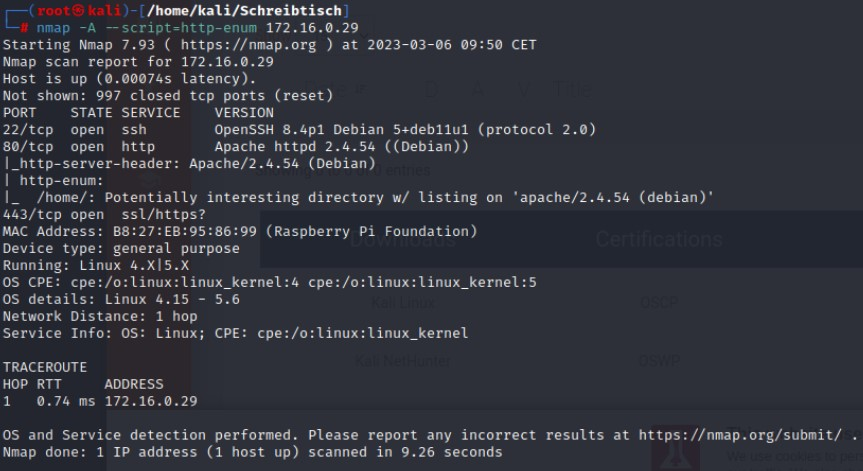
\includegraphics[width = 0.73\textwidth]{http_vulnerbility.jpg}
    \newline
    The indication that the service uses http is confirmed to be true after accessing the address 172.16.0.29:80.
	\\ 
	&\\
	&\\
    Recommendation& Use https instead to encrypt the data traffic for third parties.\\    
    \\\\\\\\\\\\\\\\\\\\\\\\\\\\\\\\\\\\\\\\\\\\\\\\\\\\\\
    \end{tabular*}
    \end{table}